\documentclass[11pt]{article}

\usepackage{amsmath,amssymb,amsfonts}
\usepackage{dsfont}
\usepackage{listings}
\usepackage{xcolor}
\usepackage{graphicx}
\usepackage{bbm}
\usepackage{float}
%\usepackage{hyperref}
\usepackage{subfig}
\usepackage[breaklinks=true,colorlinks,citecolor=black,linkcolor=gfGG,urlcolor=gfFP]{hyperref}
% http://www.colourlovers.com/palette/92095/Giant_Goldfish
\definecolor{gfCD}{HTML}{69D2E7} % Cloudless Day
\definecolor{gfSP}{HTML}{A7DBD8} % Sunken Pool
\definecolor{gfBS}{HTML}{E0E4CC} % Beach Storm
\definecolor{gfGG}{HTML}{F38630} % Giant Goldfish
\definecolor{gfFP}{HTML}{FA6900} % Food Pills

\definecolor{codegreen}{rgb}{0,0.6,0}
\definecolor{codegray}{rgb}{0.5,0.5,0.5}
\definecolor{codepurple}{rgb}{0.58,0,0.82}
\definecolor{backcolour}{rgb}{0.95,0.95,0.92}
\lstdefinestyle{mystyle}{
    backgroundcolor=\color{backcolour},
    commentstyle=\color{codegreen},
    keywordstyle=\color{magenta},
    numberstyle=\tiny\color{codegray},
    stringstyle=\color{codepurple},
    basicstyle=\ttfamily\footnotesize,
    breakatwhitespace=false,
    breaklines=true,
    captionpos=b,
    keepspaces=true,
    numbers=left,
    numbersep=5pt,
    showspaces=false,
    showstringspaces=false,
    showtabs=false,
    tabsize=2
}

\setlength{\topmargin}{-.5in} \setlength{\textheight}{9.25in}
\setlength{\oddsidemargin}{0in} \setlength{\textwidth}{6.8in}

%\newcommand*{\SOLVE}{}%

\renewcommand{\vec}[1]{\mbox{\boldmath$#1$}}
\newcommand{\mm}[1]{\mathbf{#1}}

\newcounter{ProblemNum}
\newcounter{SubProblemNum}[ProblemNum]

\renewcommand{\theProblemNum}{\arabic{ProblemNum}}
\renewcommand{\theSubProblemNum}{\alph{SubProblemNum}}

\newcommand*{\anyproblem}[1]{\section*{#1}}
\newcommand*{\problem}[1]{\stepcounter{ProblemNum} %
   \anyproblem{Problem \theProblemNum \; (#1 points)}}
\newcommand*{\soln}[1]{\subsection*{#1}}
\newcommand*{\solution}{\soln{Solution}}
\newenvironment{solutions}
  {\section[Solution]{\textcolor{red}{Solution}}\color{red}}
  {\normalcolor}
\renewcommand*{\part}{\stepcounter{SubProblemNum} %
  \soln{Part (\theSubProblemNum)}}
\renewcommand{\theenumi}{(\alph{enumi})}
\renewcommand{\labelenumi}{\theenumi}
\renewcommand{\theenumii}{\roman{enumii}}
\let\endsection\relax
\let\endsubsection\relax

\graphicspath{
{.}
}
\lstset{style=mystyle}

\begin{document}

\Large
\noindent{\bf CS4851/6851 IDL: Homework 3 \hfill \today}
\medskip\hrule

\vspace{20pt}

Note: All coding problems to be submited with Github Link. Do not Upload the files/folder. Use git commands only.

Note: this is the distribution of questions:
\begin{enumerate}

  \item Question 1 to Question 2: Required for everyone.
  \item Question 3 to Question 4:  Bonus question for both Graduate Students and Undergraduate Students
\end{enumerate}


\problem{30}
Object detection and Object Segmentation are two very important tasks in computer vision. There are many real world applications of these tasks. Take one of these tasks and explain how you would implement it. For example, Image segmentation is used in medical imaging.
\problem{30}
how does YOLO (You only Look once) works? What is the the difference between YOLO and Faster-RCNN? 
\noindent\rule[0.5ex]{0.45\linewidth}{1pt} Bonus for both  undergraduates and graduates beyond this line.
\problem{40}
In classification problem, cross entropy typically exhibits a faster convergence times than the alternatives. Consider a binary classification problem with cross binary as a loss. Note, in this case the labels are $y \in {0, 1}$ and network output of a single logistic sigmoid unit represents the conditional distribution of $k = 1$ class given data $P(k = 1 | x)$. Assume the data is i.i.d and write down the negative log liklihood that corresponds to the case when data can be mislabeled with probability $\epsilon$. Make sure that your function reduces to the convolutional cross entropy when $\epsilon = 0$. Discuss the robutness properties if any of your new loss.
\problem{40} Consider the computational graph in $\ref{fig:image_example}$. Note, that this is a simplfied version of $\textbf{ResNet}$ that we studied in class.  Write down reverse mode trace for this computation without evaluating it at a point to find dy/dx. Describe your observation of the most pronounced property of the final expression. Evaluate the gradient at x = 0. What would happen to the gradient if there was no skip connection from x to y. 
This exercise is to understand how gradients flow in a skip connection network and how we can encounter vanishing gradient issues if any.

\begin{figure}[t]
\begin{center}
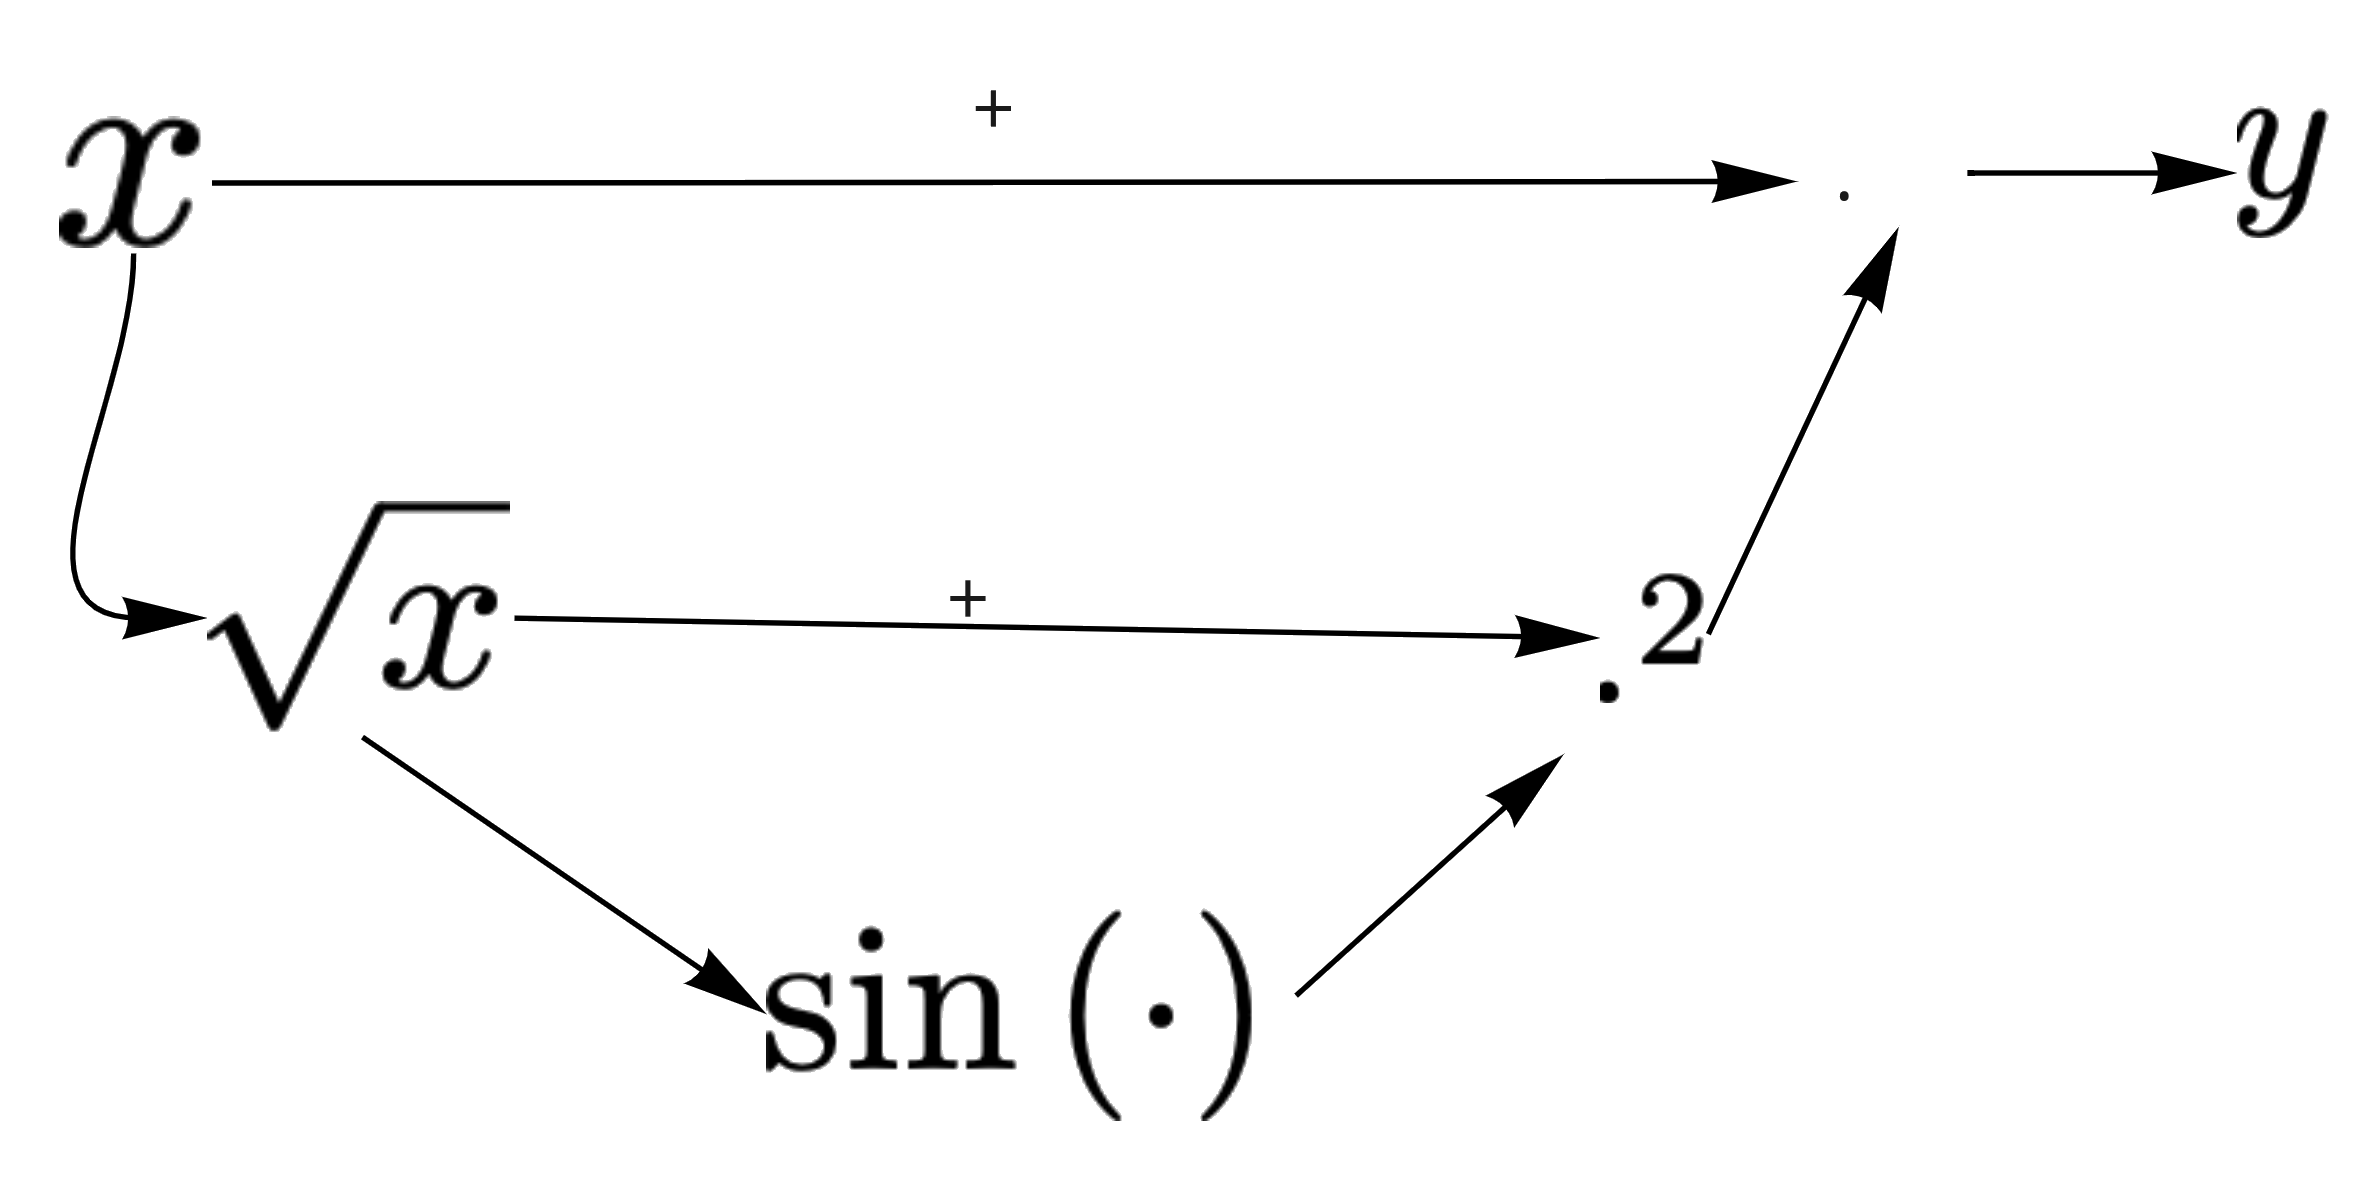
\includegraphics[width=1.0\textwidth]{unet.png}
\end{center}
\caption{Resnet}
\label{fig:image_example}
\end{figure}
% \vspace{2px}
\end{document}

%%% Local Variables:
%%% mode: latex
%%% TeX-master: t
%%% End:

